\documentclass[12pt,english]{scrartcl}

\usepackage{amsmath,amssymb}
%\usepackage[amssymb]{SIunits}
\usepackage{babel}
\usepackage[latin1]{inputenc}
\usepackage{graphicx}
\usepackage{color}

\title{KOGW-PM-KNP: Tutorial 10 - Signal Detection Theory}
\author{}
\date{\today}

\begin{document}

\maketitle

\centering
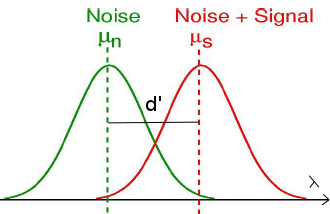
\includegraphics[scale=0.5]{SDT_fig1.png} 
\begin{enumerate}
\item \textbf{Noise and Signal and Noise Distribution} \\

Plot the noise and signal+noise distributions for different sensitivity, $d$, values: [0.25, 0.5, 1.0, 3.0, 7.0]. Generate these distributions across a range of  +4 -4. \\

Also, plot the criterion for five different values of $\lambda$, with $\lambda$ being equally spaced between and . \\

It is often assumed that the decision axis values, x, are distributed normally and with equal variance in noise $(S = 0)$ and signal $+$ noise trials $(S = 1)$. With $S = 0, X  N(0, 1)$ and with $S = 1, X  N(d,1)$ \\

\textit{Hint: Use the stats.norm.pdf function to generate your distribution. And matplotlib.pyplot.plt for plotting}

\color{black}
\item \textbf{Hits, False Alarms and ROC-curves} \\
 
Plot the theoretically derived ROC-curves (hits vs. false alarms) for the sensitivity, d, and criterion, λ, combinations described above. Use the same color for points that lie on one ROC-(isosensitivity-)curve.

\textit{Hint: Use the stats.norm.cdf function to generate your cumulative distribution.}
  
\color{black}
\item \textbf{Nonstandard normal distributions (Add-on)} \\
Solve the problems b-g of Exercise 1.4 in the Analytical Tutorial with the programming routines you just developed.
   

\end{enumerate}
 \color{black}
 Maximum marks 10/10 \\

\end{document}